\section{Downloading data from the GRID}\label{apx:Downloading_Data}
\begin{minted}{bash}
    # The directory in alimonitor where you want to get the data from. Should contain a load of numbered directories
    # For example, /alice/data/2021/OCT/505548/AOD. Note that it's AOD not AO2D
    sourceMotherDir=/alice/data/path/to/AOD
    nFiles=$1

    # This is the directory on your local machine where you want to store your data
    targetMotherDir=/path/to/alice/data/${sourceMotherDir}
    mkdir -p ${targetMotherDir}

    for ((i=1; i<=nFiles; i++))
    do
        if (( i < 10 )); then
            pref=00
        fi
        if (( i > 9 )); then
            pref=0
        fi
        iDir=${pref}${i}
        iSourceDir=${sourceMotherDir}/${iDir}
        iTargetDir=${targetMotherDir}/${iDir}
        mkdir -p ${iTargetDir}

        echo "copying from ${iSourceDir} to ${iTargetDir}" 
        
        alien_cp -retry 5 ${iSourceDir}/AO2D.root file://${iTargetDir}/AO2D.root
    done
\end{minted}

\newpage
\section{Additional Plots}\label{apx:Additional_Plots}

\begin{figure}[h]%
    \centering
    \begin{subfigure}[t]{.49\linewidth}
        \centering
        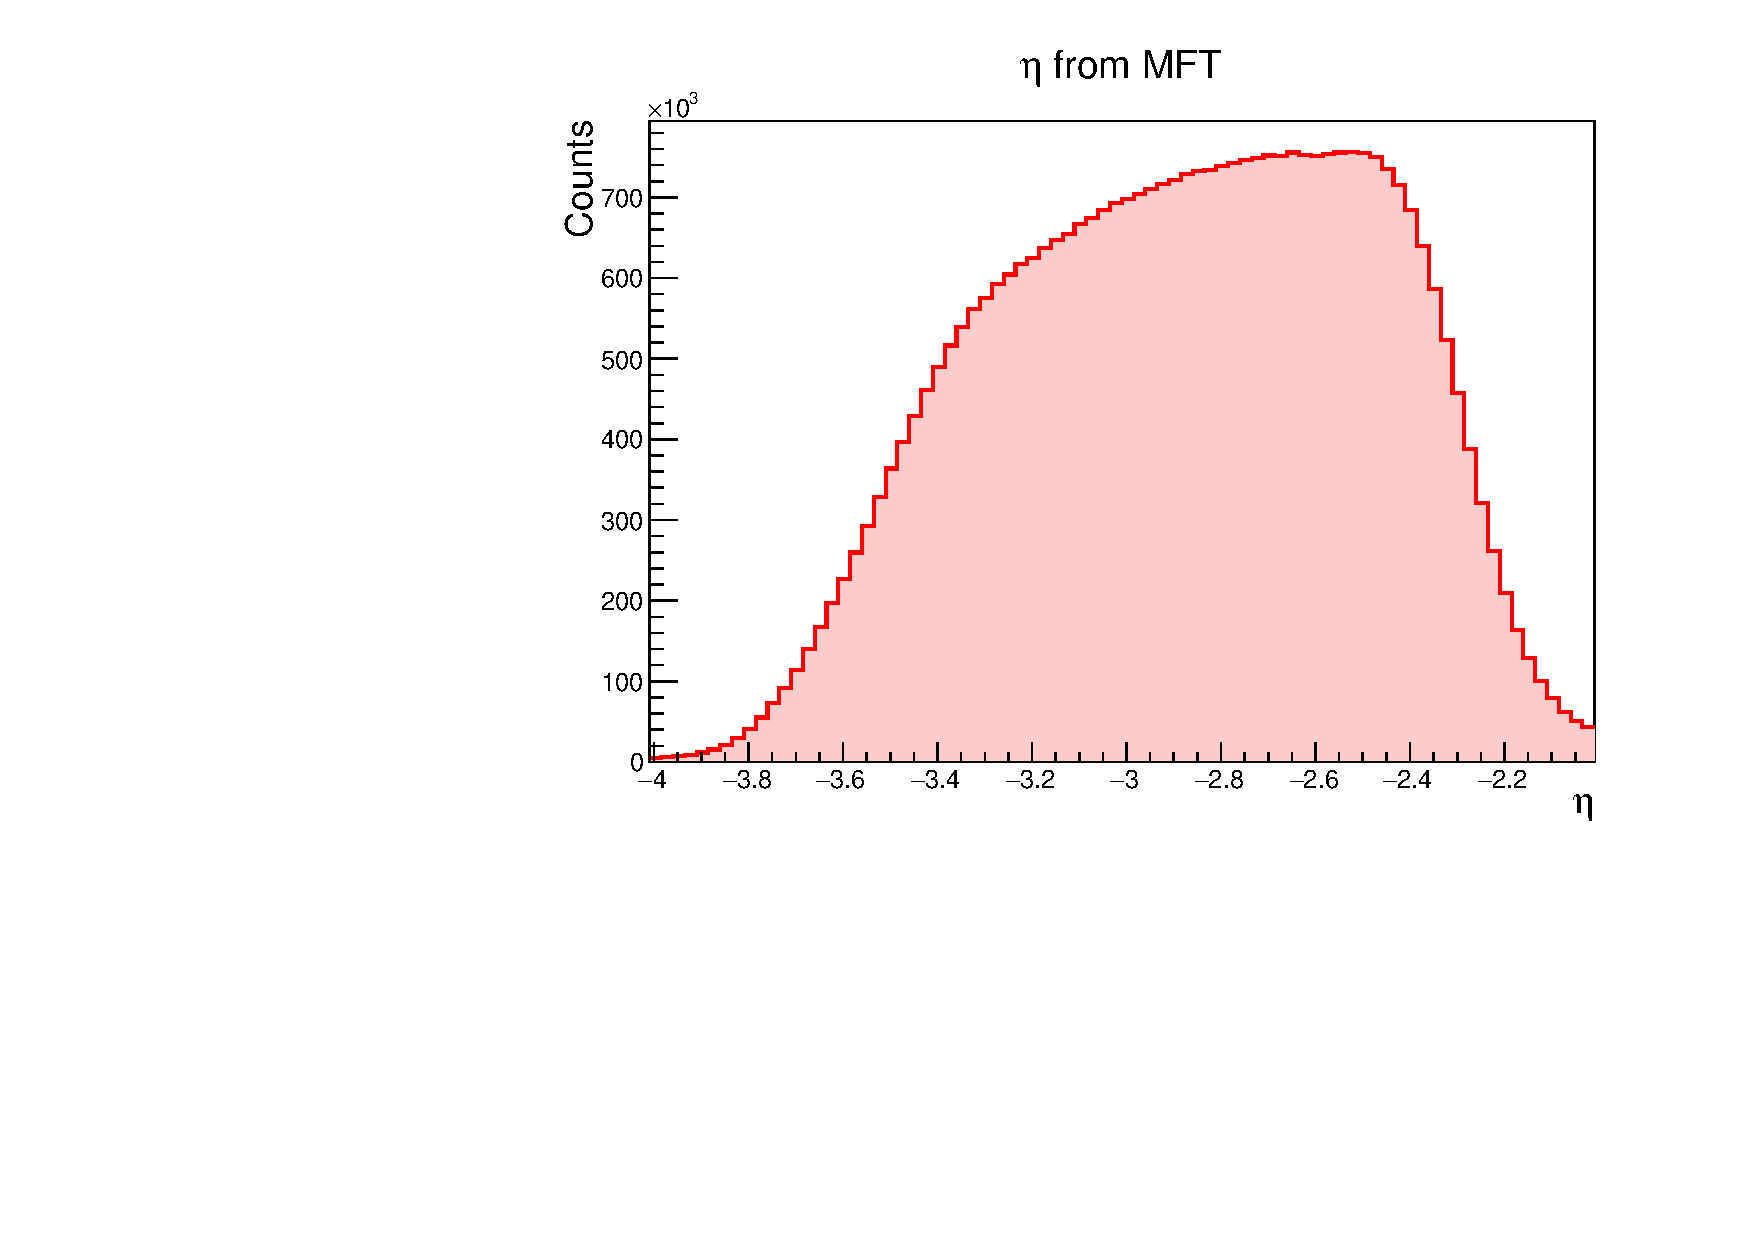
\includegraphics[width=\linewidth]{Plots/pass4_MFT/MFTeta_pass4.pdf}
        \caption{}
        \label{}
    \end{subfigure}
    \hfill
    \begin{subfigure}[t]{.49\linewidth}
        \centering
        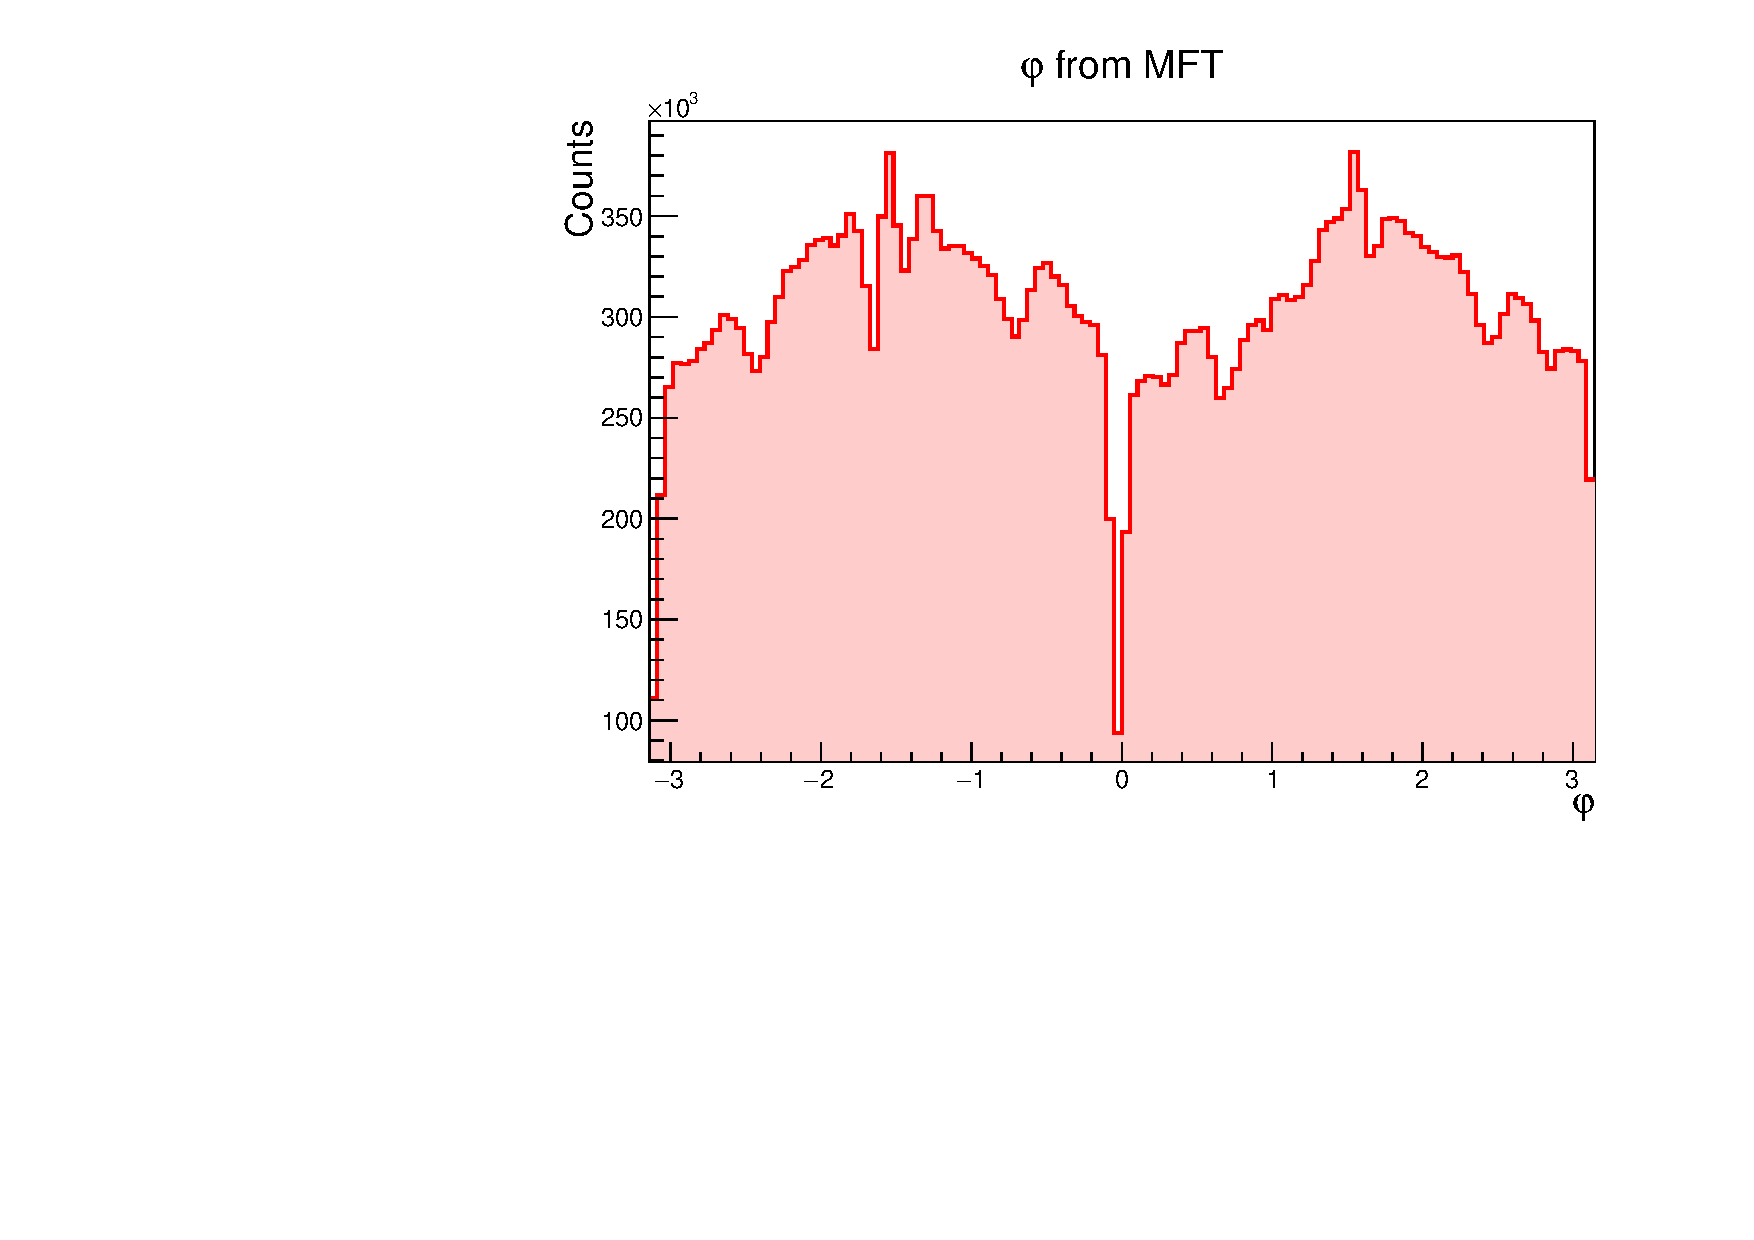
\includegraphics[width=\linewidth]{Plots/pass4_MFT/phi_pass4.pdf}
        \caption{}
        \label{}
    \end{subfigure}
    \begin{subfigure}[t]{.49\linewidth}
        \centering
        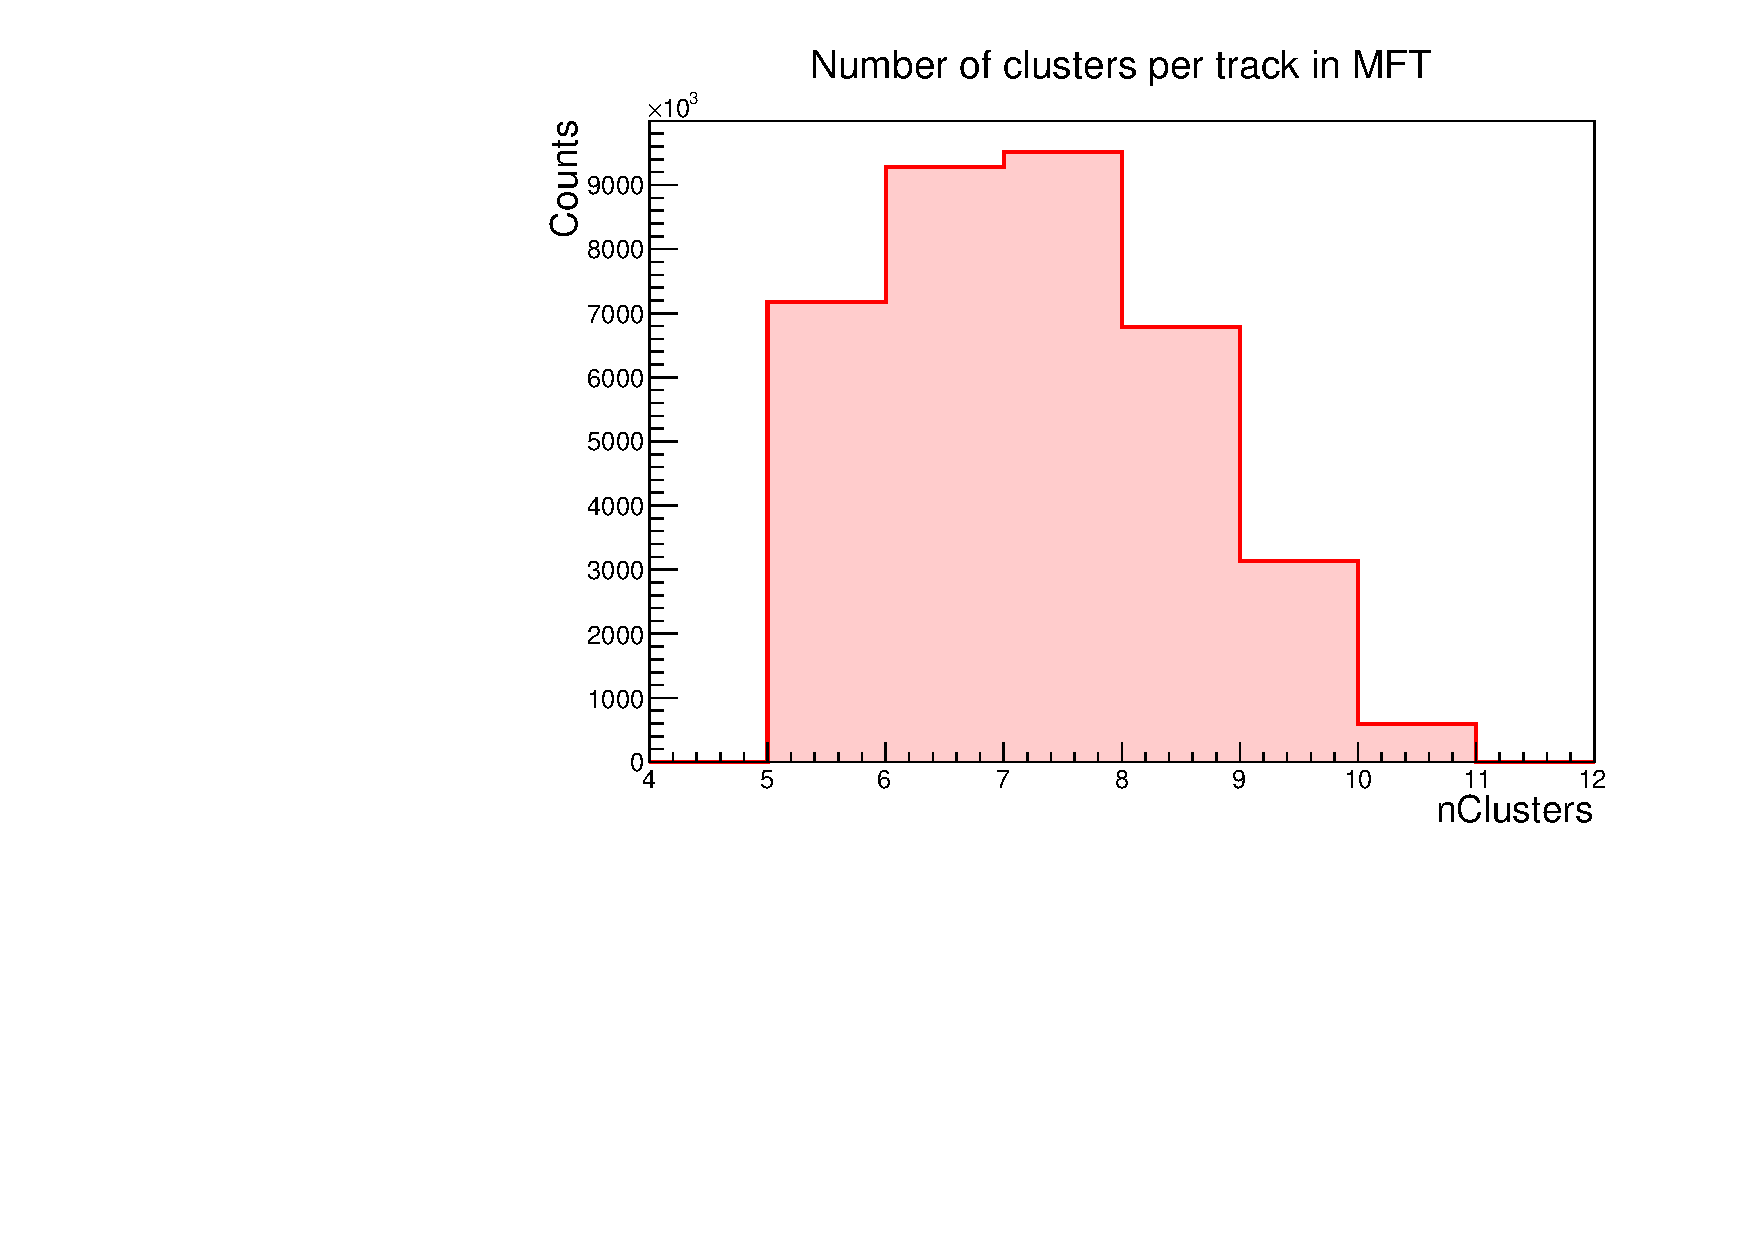
\includegraphics[width=\linewidth]{Plots/pass4_MFT/nClusters_pass4.pdf}
        \caption{}
        \label{}
    \end{subfigure}
    \hfill
    \begin{subfigure}[t]{.49\linewidth}
        \centering
        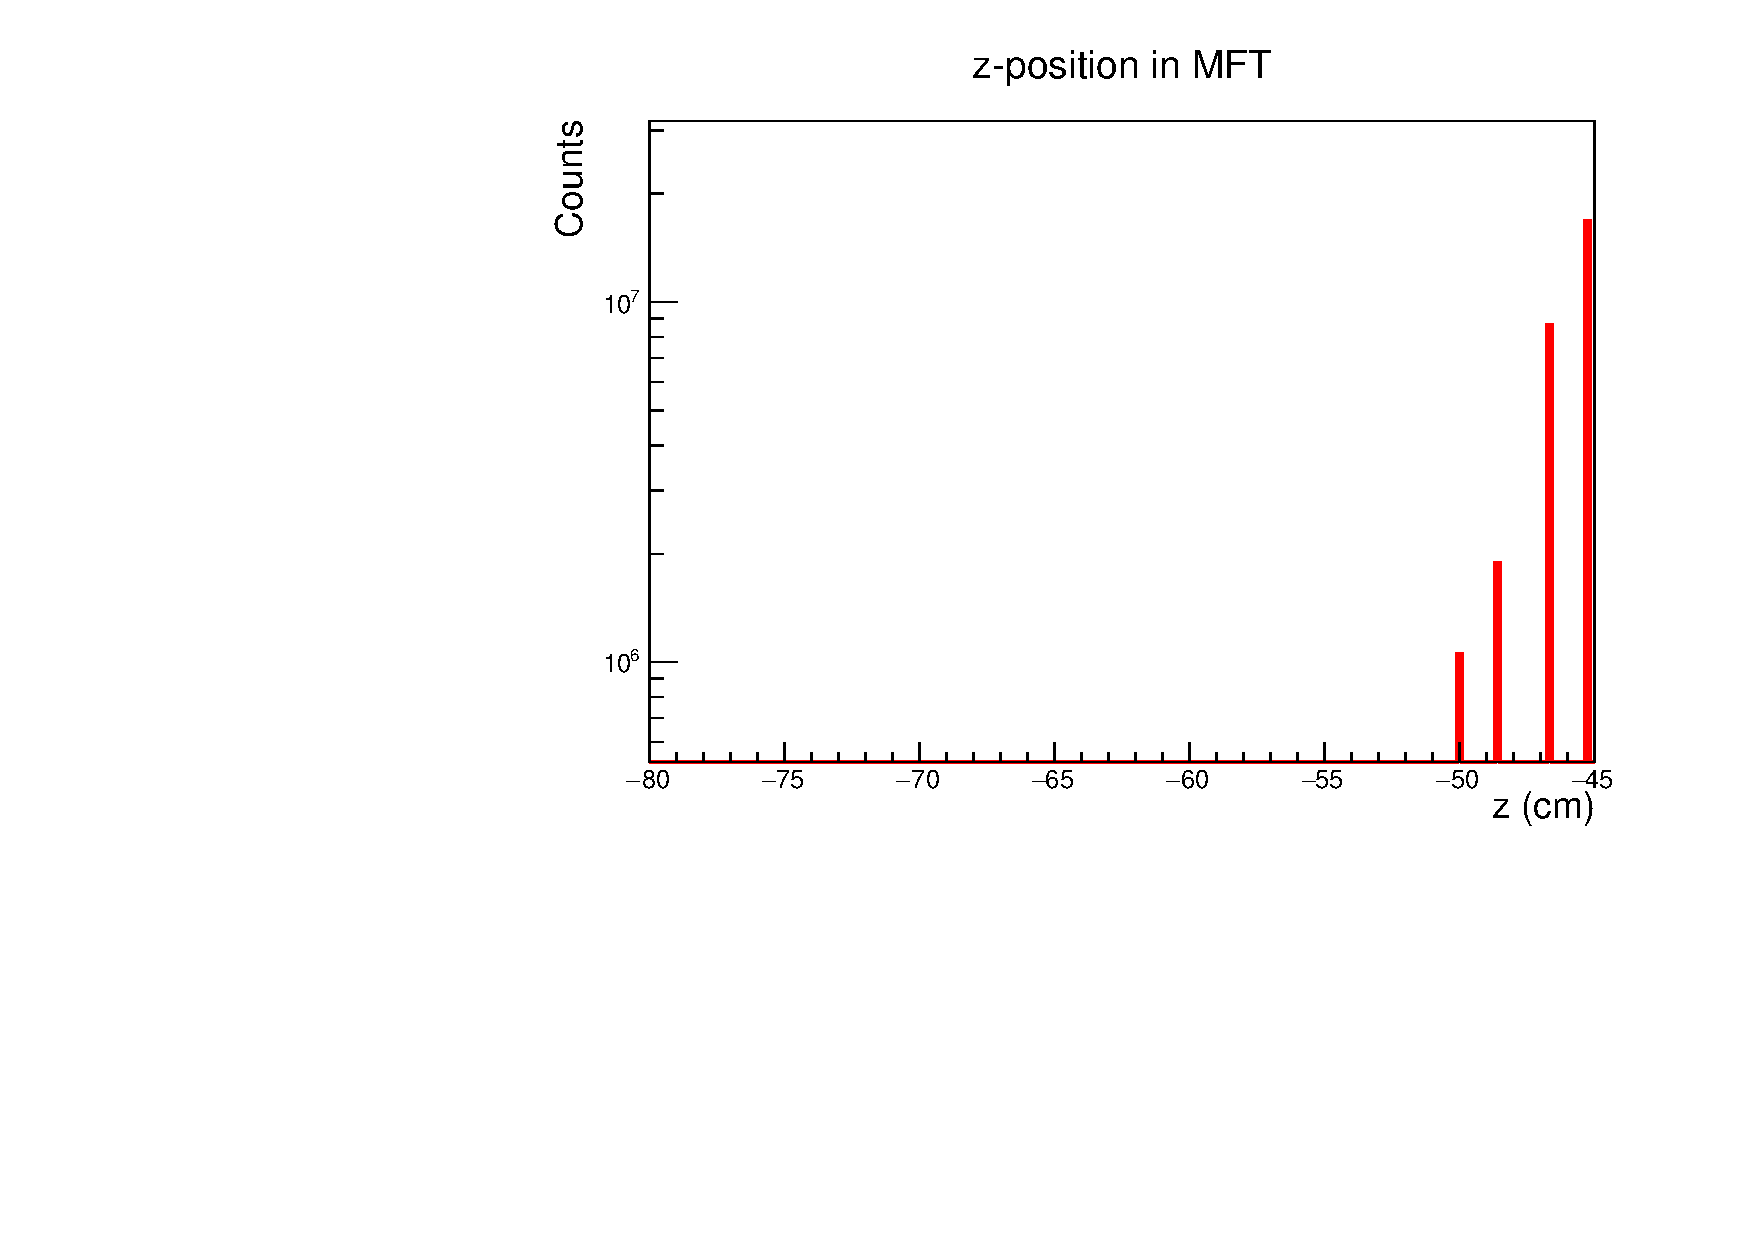
\includegraphics[width=\linewidth]{Plots/pass4_MFT/Z_MFT_pass4.pdf}
        \caption{}
        \label{}
    \end{subfigure}
\caption[Histograms of $\eta$, $\varphi$, \OldTexttt{nClusters}, and $z$ for tracks from pass 4 in the MFT]{Histograms of kinematic variables for tracks in the MFT from reconstruction pass 4. Presented here for comparison to \cref{fig:MFT_1D_pass3}. Note that other than $\eta$ there is no significant difference between these and those from pass 3. }
\label{fig:MFT_1D_pass4}
\end{figure}

\begin{figure}[h]%
    \centering
    \begin{subfigure}[t]{.49\linewidth}
        \centering
        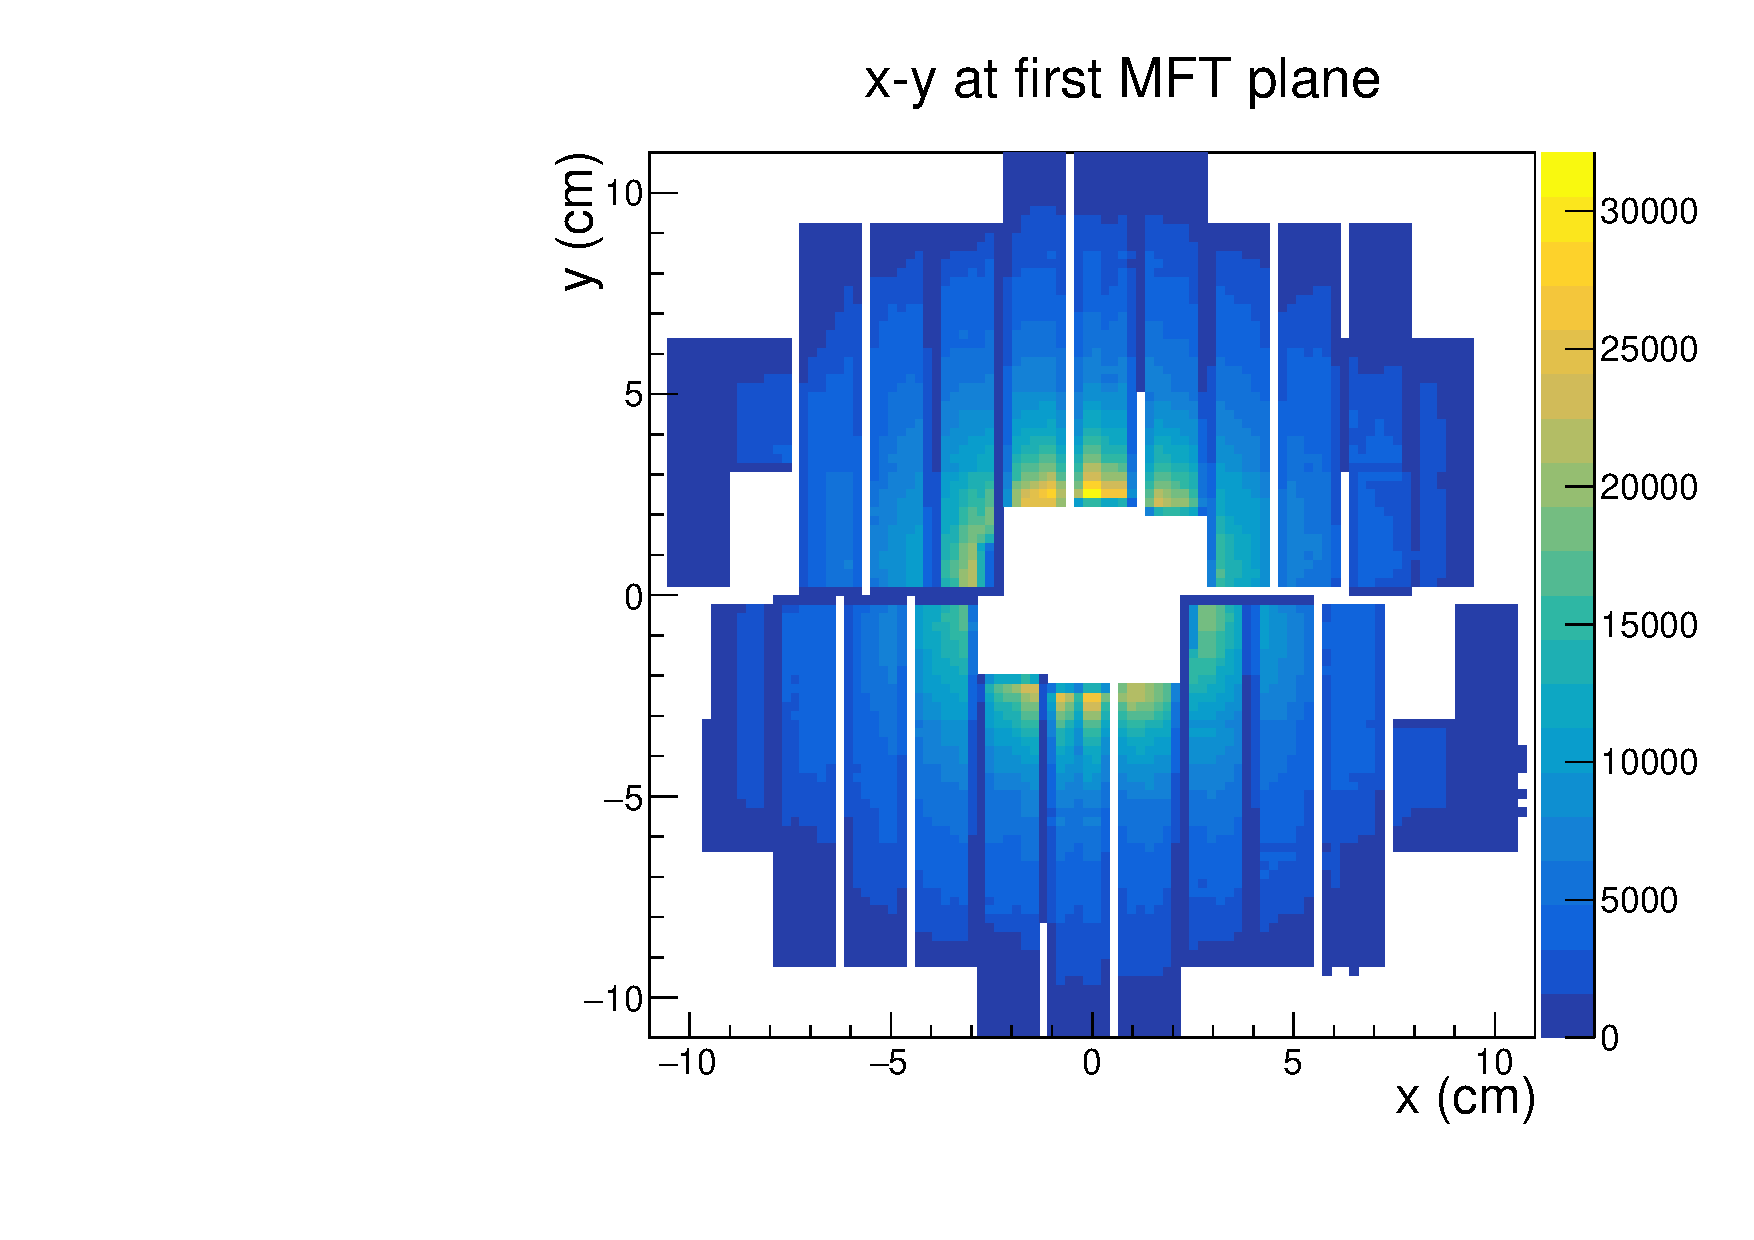
\includegraphics[width=\linewidth]{Plots/pass4_MFT/x_y_1_pass4.pdf}
        \caption{}
        \label{}
    \end{subfigure}
    \hfill
    \begin{subfigure}[t]{.49\linewidth}
        \centering
        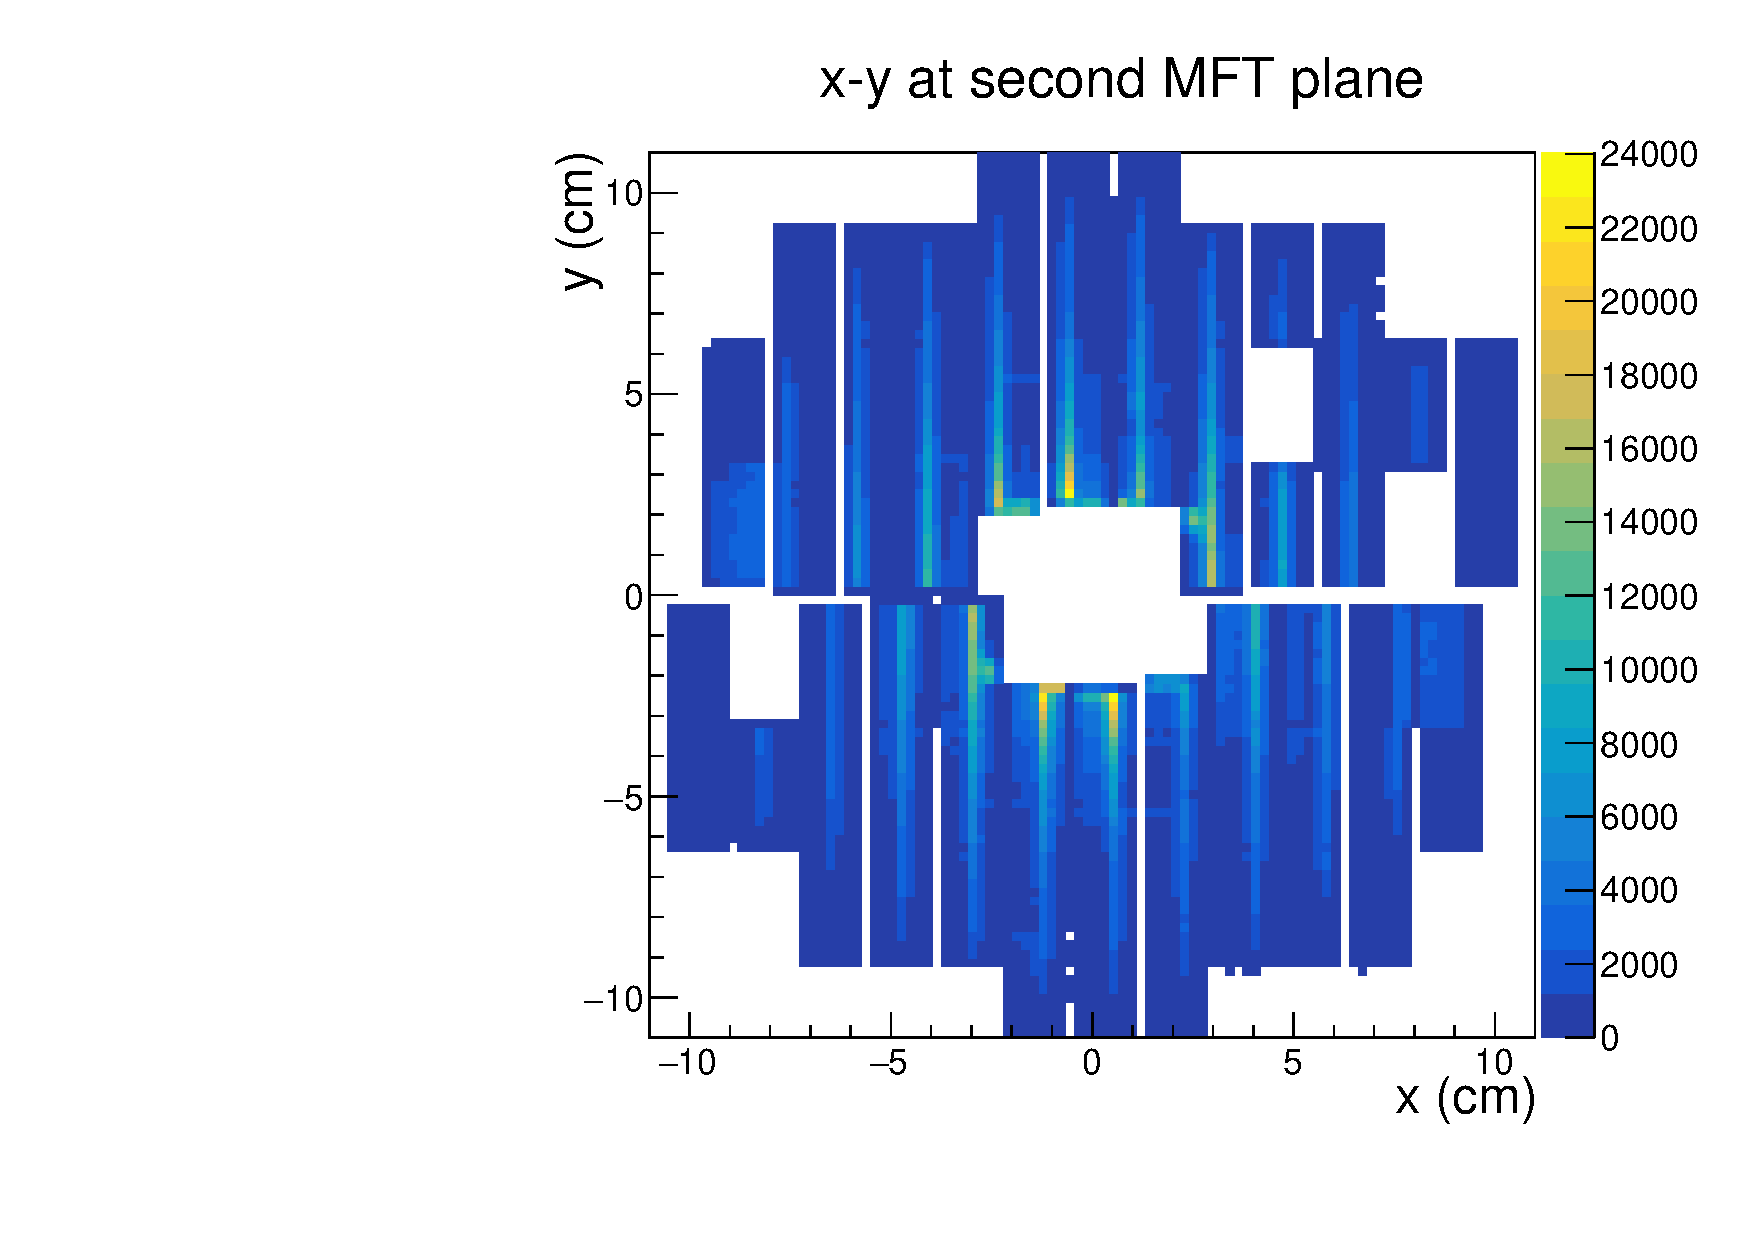
\includegraphics[width=\linewidth]{Plots/pass4_MFT/x_y_2_pass4.pdf}
        \caption{}
        \label{}
    \end{subfigure}
    \begin{subfigure}[t]{.49\linewidth}
        \centering
        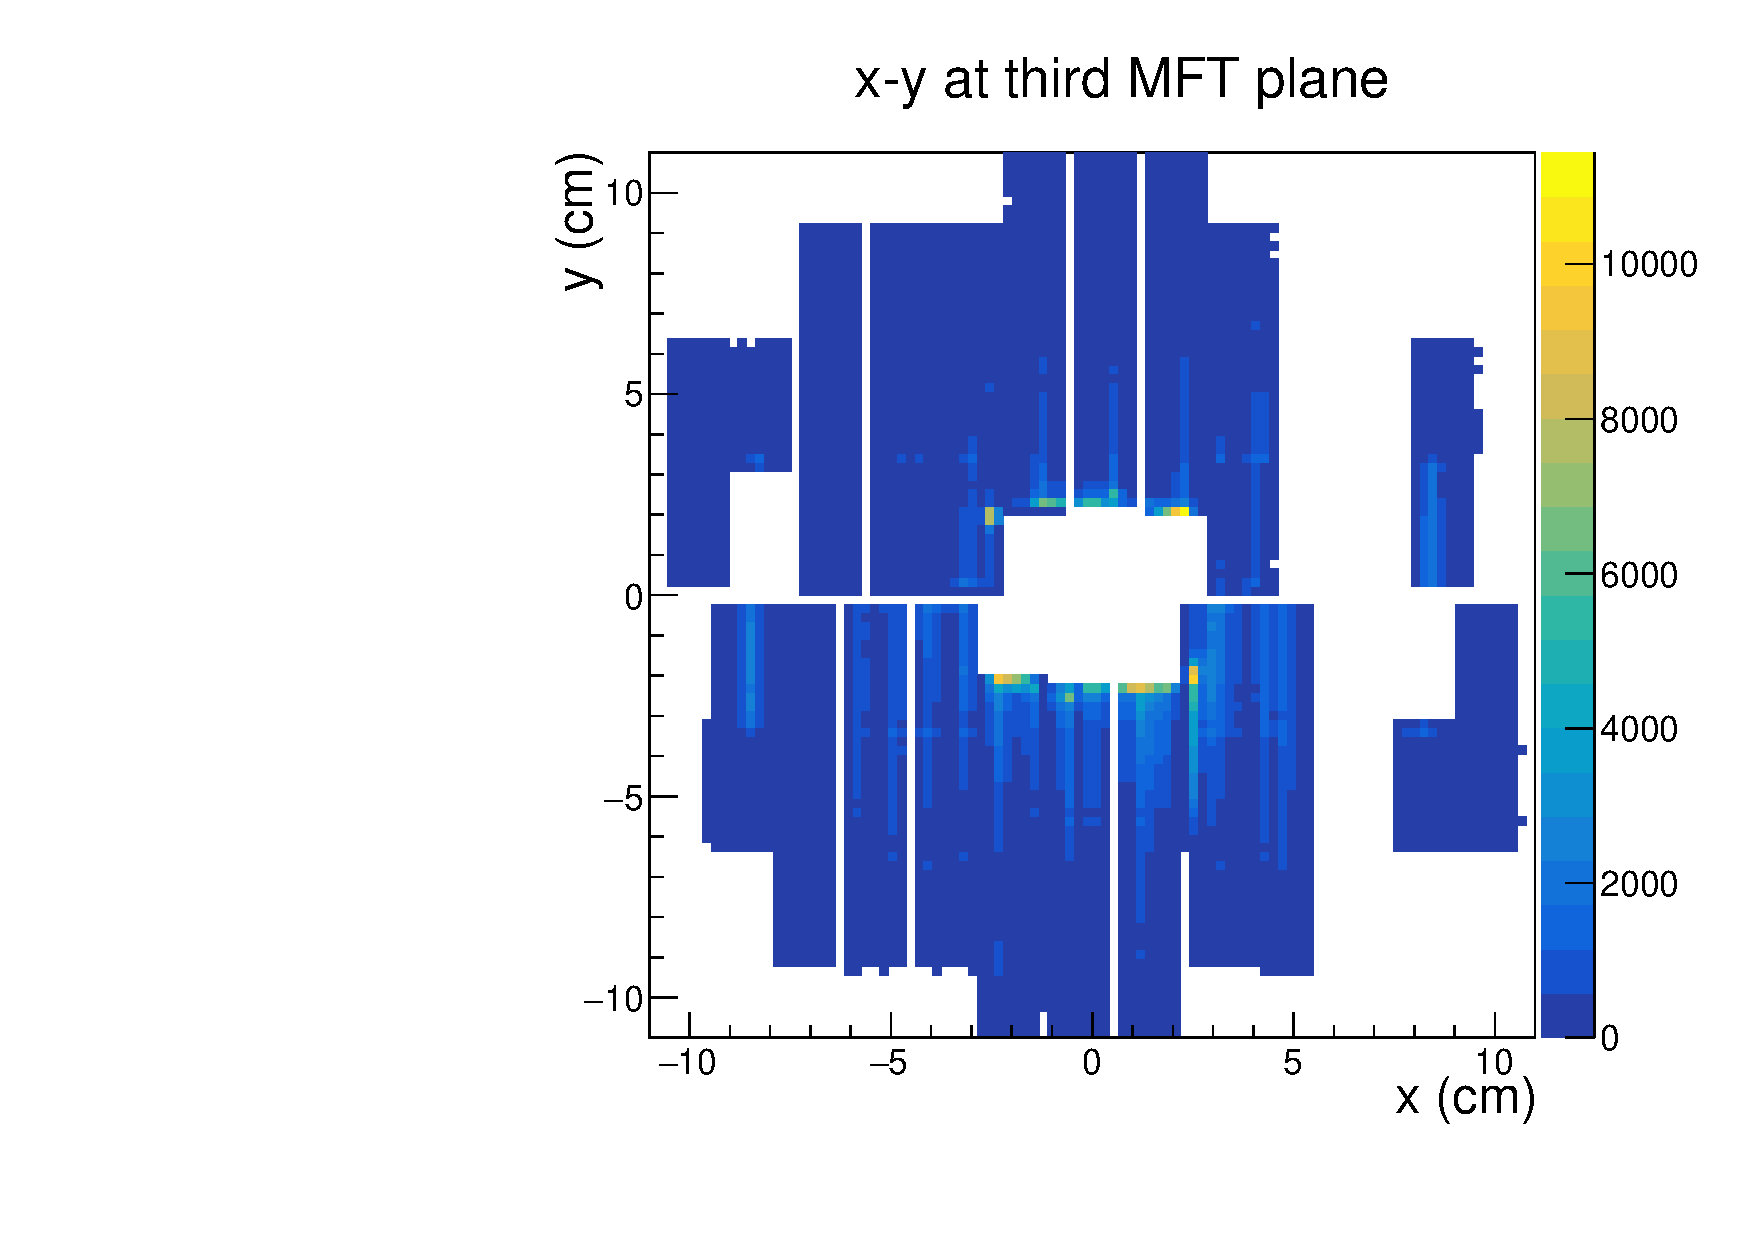
\includegraphics[width=\linewidth]{Plots/pass4_MFT/x_y_3_pass4.pdf}
        \caption{}
        \label{}
    \end{subfigure}
    \hfill
    \begin{subfigure}[t]{.49\linewidth}
        \centering
        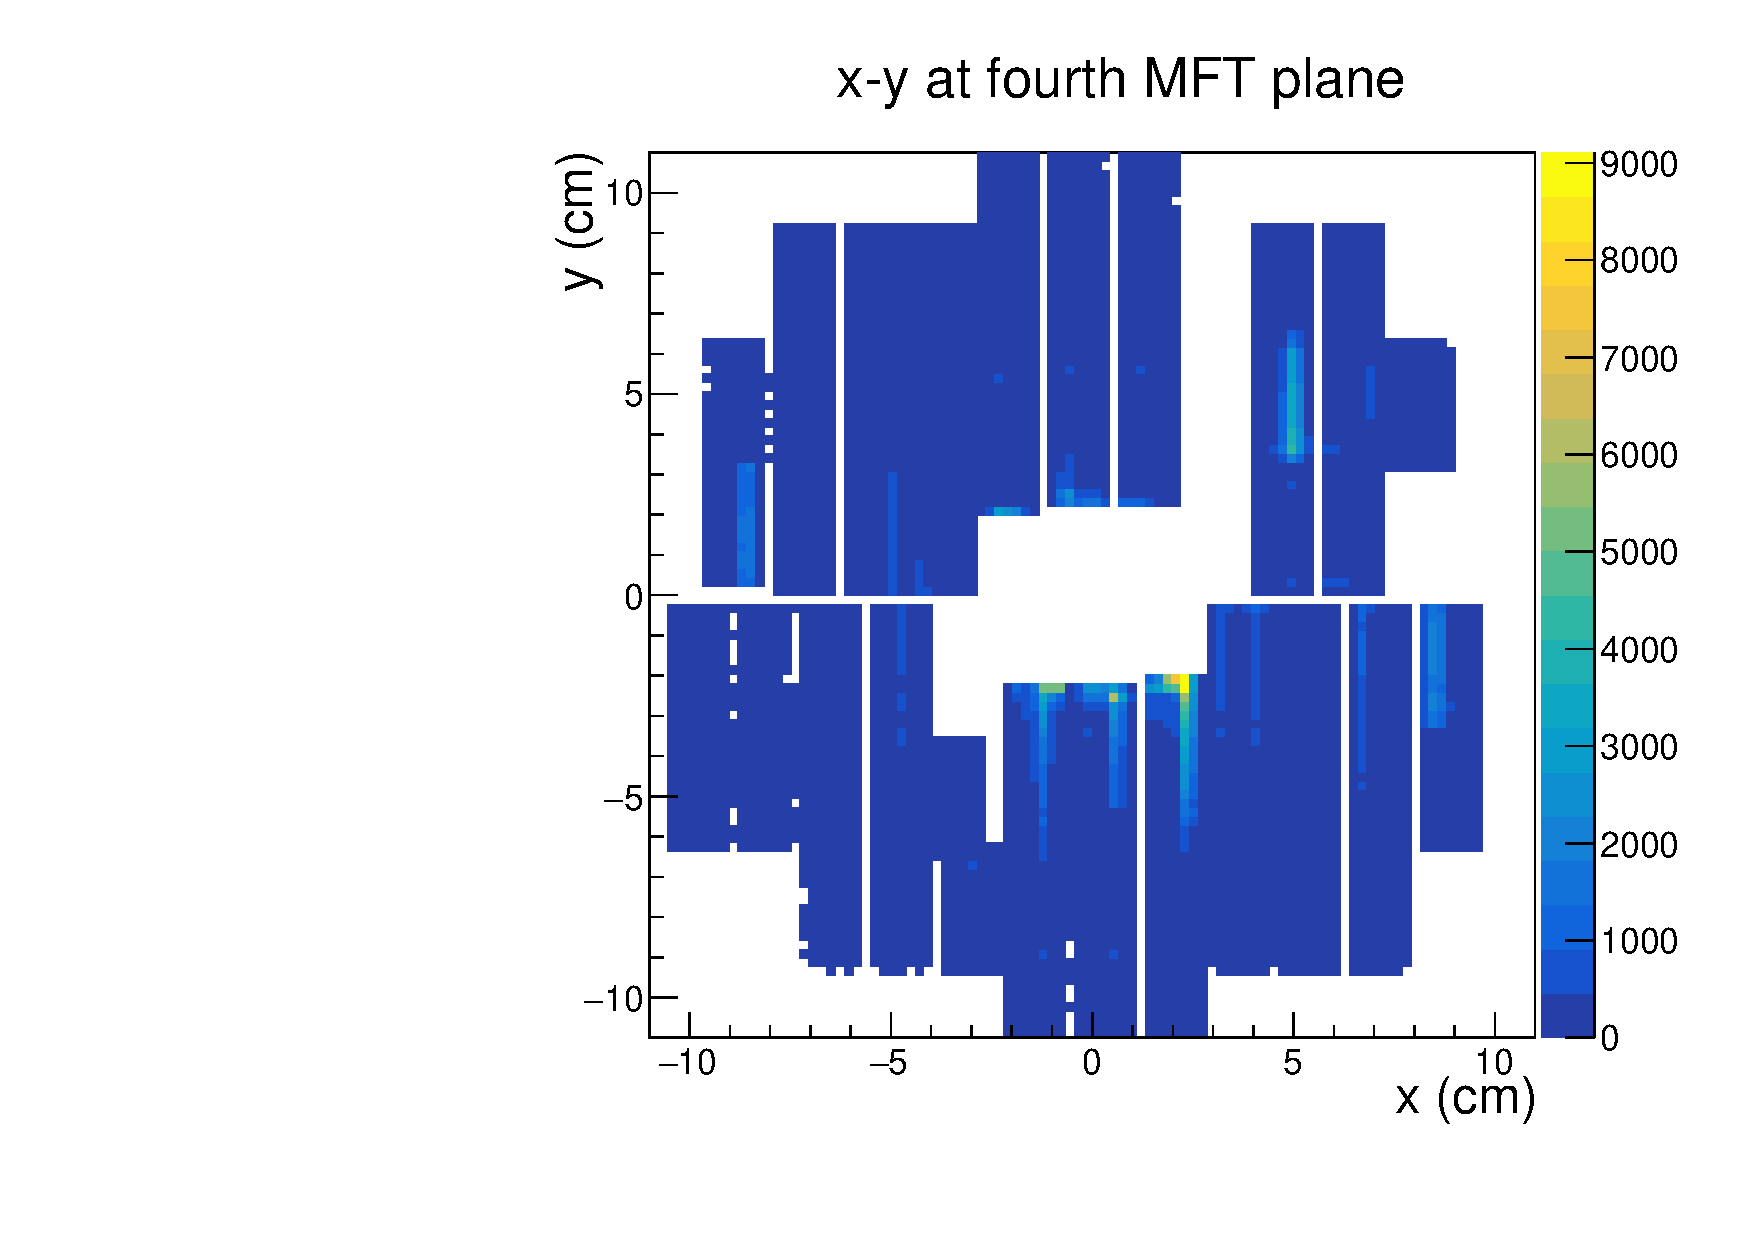
\includegraphics[width=\linewidth]{Plots/pass4_MFT/x_y_4_pass4.pdf}
        \caption{}
        \label{}
    \end{subfigure}
\caption[$x$-$y$ histograms of tracks at different planes in the MFT]{$x$-$y$ histograms for MFT tracks from reconstruction pass 4. Once again there is not much difference compared to pass 3 other than a general trend towards more uniform data. }
\label{fig:MFT_2D_pass4}
\end{figure}